\chapter{LHC and \gls{atlas}}
\label{chap:cern}

The analyses presented in this thesis use the \gls{pp} collision data at a center-of-mass energy \cmtre TeV 
collected by the \gls{atlas} experiment in 2015, 2016 and 2017. 

The \gls{atlas} experiment is one of the four main experiments at the \gls{lhc} at the \gls{cern}. Section \ref{sed:cern:lhc} of this chapter describes the \gls{lhc} accelerator complex. This is followed by a general description of the detectors used in high-energy physics in Section \ref{sec:detectors}. The \gls{atlas} detector is discussed in Section \ref{sed:cern:atlas}.

%%%%%%%%%%%%%%%%%% LHC

\section{The Large Hadron Collider}
\label{sed:cern:lhc}

In this section we give a brief introduction to the \gls{lhc} \cite{1748-0221-3-08-S08001}, at the moment the largest and most powerful particle accelerator in the world, hosted by \gls{cern} and in operation since September 2008.


\subsection{A circular hadron collider}

The \gls{lhc} is a circular hadron accelerator, located in a 26.7-km-long underground tunnel (with a depth ranging between 50 and 140 meters) that was previously hosting the \gls{lep}, a \gls{cern} accelerator that was operational from 1989 to 2000. The \gls{lhc} can accelerate protons up to a design center-of-mass energy of 13 TeV. Accelerating particles to very high energies is necessary both to study the structure of the particles themselves at smaller scales, and to create heavy states in collisions. Cosmic rays provide a source of particles with energies up to $10^7$ times more than what the \gls{lhc} is capable of, but these extremely energetic rays are very rare, and the flux is not controlled. Accelerators provide a well controlled flux of particles of a specific type in a specific location, and this allows the study of these particles with dedicated detectors.

A circular accelerator simplifies the acceleration of particles, as this can happen over several revolutions. When a charged particle travels on an orbit of radius $r$ under the effect of a magnetic field $B$, its momentum $p$ is given by:
\begin{equation}
\label{eq:cern:p03br}
p = 0.3 r B,
\end{equation}
\noindent where the momentum is expressed in GeV, B in Tesla and the radius of the orbit in meters. For a given magnetic field, a larger radius allows to reach higher energies. 

The choice of a collider over a fixed-target experiment is motivated by the possibility of reaching a higher energy in center-of-mass of the system: while in a fixed-target experiment this is proportional to the square root of the energy of the incoming particle, in a collider it is the sum of the energies of the two beams.


Suitable particles for a collider experiment need to fulfill two criteria: they need to be charged, in order to be accelerated and guided through electric and magnetic fields, and they need to be stable enough not to decay before being used for collisions. These criteria effectively limit the choice to protons, electrons, their antiparticles and ions. 

At the \gls{lhc} it has been chosen to study collisions with protons and lead ions. Three types of collisions are studied: proton-proton ($p-p$), lead-lead ($Pb-Pb$) and also proton-lead ($Pb-p$). The main reason to prefer protons over electrons is the energy loss that affects charged particles accelerated in a circular trajectory (\textit{syncrotron radiation}), which decreases with the fourth power of the mass of the particle:

\begin{equation}
\label{eq:cern:sync}
\frac{dE}{dt} \propto \frac{E^4}{m^4 r^2} \; .
\end{equation}

The larger mass of a proton with respect to an electron leads to a decrease by a factor $10^{12}$ in the energy lost through syncrotron radiation. This choice comes with a price: proton-proton collisions lead to less clean events, with a lot of soft interactions covering the interesting hard interactions. Furthermore, the center-of-mass energy is unknown as the particles taking part in hard interactions are not the protons themselves but their constituents.

\subsection{Magnet system} 


The \gls{lhc} is not a perfect circumference: it is composed of eight arcs (\textit{sectors}), where the magnetic system is located, and eight straight sections containing the resonant cavities, the four interaction points with and the detectors, the equipment for beam injection and extraction, and other instrumentation. Magnetic fields are used to govern the trajectory of the particles. In the \gls{lhc} there are more than nine thousand magnets, constructed from a superconducting alloy of niobium and titanium. About 150 tons of super-fluid helium at a temperature of 1.9 K are used to maintain the magnet system in the superconducting regime. Different types of magnets are necessary to achieve a proper control over the trajectory of the particles.

\subsubsection*{Dipoles} 
Dipoles are used to create a vertical magnetic field, so as to bend the particles in the horizontal plane and thus give the dominant circular orbit. The \gls{lhc} has 1232 dipoles, each 15 m long and providing a magnetic field of 8.3 T. The current necessary to achieve this strong magnetic field is 11.8 kA.


\subsubsection*{Quadrupoles}
The \gls{lhc} has 858 quadrupoles, used for beam focusing. A single quadrupole can focus the beam either in the vertical or the horizontal plane, but it causes a defocusing in the other plane; conventionally a quadrupole is denoted as focusing if it is oriented to focus in the horizontal plane. A combination of focusing and defocusing quadrupoles separated by some drift space (\textit{FODO lattice}) is used to keep both planes focused, and gives rise to \textit{Betatron oscillations}. Figure \ref{fig:lhc:quad} shows a schematic representation of the transverse view of a quadrupole magnet.

\subsubsection*{Higher-order magnets} 
Beside dipoles and quadrupoles, in the \gls{lhc} there are about 600 higher-order magnets that are used to maintain a good beam quality; e.g.  sextupoles are used to correct the spread in Betatron tune caused by the quadrupoles.




\begin{figure}[ht]
\centering
\includegraphics[width=0.45\textwidth]{figures/lhc/figures_quad}
\caption{A schematic cross-section of a quadrupole magnet. The red arrows indicate the direction of the force experienced by the particle. Figure from Ref. \cite{Kain:2016aly}.}
\label{fig:lhc:quad}
\end{figure}

\subsection{Resonant cavities}

While the orbit of particles is governed by the magnetic fields, longitudinal electric fields are used for acceleration. In the \gls{lhc} the electric filed is provided by \gls{rf} cavities. There are overall 16 \gls{rf} cavities, eight per beam, hosted in four cryo-modules. Each cavity can provide an accelerating field of 5 MV/m, and oscillates with a frequency of 400 MHz. Since the electric field changes over time with the oscillations, particles passing through the same point of a \gls{rf} cavity at different times experience a different voltage; this produces a non-trivial longitudinal dynamics, where particles oscillate around the ideal synchronous particle with changes in momentum and phase (\textit{Synchrotron oscillations}). If we define the \textit{slip factor} $\eta$ as the relative change in frequency in Synchrotron oscillations with the relative change in momentum:
\begin{equation}
\eta = \frac{\Delta f / f}{\Delta p / p} \; ,
\end{equation}

\noindent and the compaction factor $\alpha$ as the relative change in frequency in orbit length with the relative change in momentum:

\begin{equation}
\alpha = \frac{\Delta L / L}{\Delta p / p} \; ,
\end{equation}

\noindent the following relation holds:

\begin{equation}
\eta = \frac{1}{\gamma^2} - \alpha \; ,
\end{equation}

where $\gamma$ is the Lorentz factor of the particle. This means that while the energy of the particle is low ($\eta>0$) an increase in momentum leads to an increase in frequency, while it leads to a decrease in frequency for $\eta<0$. At the transition energy, a previously stable synchrotron phase becomes unstable and vice versa; this requires a rapid change in \gls{rf} phase. This situation is illustrated in Figure \ref{fig:lhc:phase}(a). For example, a particle corresponding to the phase point M1 will arrive in the \gls{rf} cavity after one corresponding to the stability point P1, and will experiment higher voltage and increase in momentum; if $\eta>0$ this increase in momentum will translate in an increase in frequency and the particle will, at the following revolution, arrive earlier, while if $\eta<0$ the frequency will further decrease and the particle will be eventually lost.  The transition energy in the \gls{lhc} is 53 GeV, well below the injection energy of 450 GeV, so the \gls{lhc} is always above transition. 

\begin{figure}[ht]
\centering
\subfigure{\includegraphics[width=0.547\textwidth]{figures/lhc/phase-stability-2}}
\subfigure{\includegraphics[width=0.44\textwidth]{figures/lhc/bucket}}
\caption{(a) Phase stability below and above transition. Figure from Ref. \cite{Tecker:2016mlq}. (b) Bucket and the bunch for a beam above the transition energy. Figure from Ref. \cite{Baird:1017689}.}
\label{fig:lhc:phase}
\end{figure}


In the \gls{lhc} beams particles are not distributed continuously, as this would now be allowed by phase instabilities, but are divided in \textit{bunches}. 
The areas of stable motion are identified as \textit{bucket}, and the area of the bucket is the beam \textit{longitudinal acceptance}. The beam bunches fill only a part of the bucket, and the area of the beam bunches is the \textit{longitudinal beam emittance}. Figure \ref{fig:lhc:phase}(b) shows a schematic view of the bucket and the bunch area for the case of a beam above the transition energy. 

\subsection{Luminosity and operational parameters}

The amount of data delivered by an accelerator is quantified by the \textit{integrated luminosity} $\mathcal{L}_{int}$.
Given a certain process with production cross section $\sigma$, the total number of events for that process is the product of cross section and integrated luminosity:

\begin{equation}
\label{eq:cern:nev}
N_{\mathrm{events}} = \sigma \,\, \mathcal{L}_{int} \; .
\end{equation}

The integrated luminosity is the time integral of the \textit{instantaneous luminosity} $\mathcal{L}$, 

\begin{equation}
\label{eq:cern:intlumi}
\mathcal{L}_{int} = \int \mathcal{L} \, dt \; ,
\end{equation}

\noindent which, assuming a Gaussian particle distribution and the same characteristics for the two beams, can be expressed as:

\begin{equation}
\mathcal{L}=\frac{f N_b n^2}{4 \pi \sigma_{x}\sigma_{y} } \; ,
\label{eq:cern:lumi}
\end{equation}

\noindent where $f$ is the revolution frequency, $N_b$ the number of bunches in each beam, $n$ the number of protons in each bunch and $\sigma_{x(y)}$  is the transverse beam size at the interaction point in the $x$($y$) direction . 

The instantaneous luminosity defined in Eq. \ref{eq:cern:lumi} needs to be corrected for two effects. First of all, this formula assumes a head-on collision between the bunches; in reality, to avoid unwanted interactions the beams collide with a crossing angle, and a large crossing angle decreases the instantaneous luminosity. The second correction is related to the beam transverse size, that can be expressed as:
\begin{equation}
\sigma_{x,y} = \sqrt{  \epsilon \beta^* } \; ,
\end{equation}
where $\epsilon$ is the beam emittance and $\beta^*$ is the \textit{beta function}. Beam collisions happen in \textit{minibeta insertions}, drift spaces with a beta waist in the center, where the beam size is as small as possible. In the vicinity of the minimum, the beta function evolves like:

\begin{equation}
\beta(s) = \beta^* + \frac{s^2}{\beta^*} \; .
\end{equation}

From this it is possible to see that the smaller the beta function, the larger the dependence with $s$, so a bunch with a finite size will not have the same beta function as a whole (\textit{hour glass effect}). This correction becomes more important with the decrease of the $\beta^*$ value. With the \gls{lhc} design parameters, the effect of crossing angle and hour glass changes the instantaneous luminosity by about 20\%.

The main limitations in the choice of the parameters that regulate the luminosity are \textit{collective effects}, which could cause beam instabilities if the number of bunches or the number of protons per bunch is too high, and the limitations in the available aperture in the minbeta quadrupoles, that impacts $\beta^*$. The summary of the \gls{lhc} operational parameters during Run 2 is reported in Table \ref{tab:lhc:param}.


\begin{table}[ht]
\begin{center}
\begin{tabular}{c c c c c }
\hline 
Parameter & 2015 & 2016 & 2017 & Design \\ 
\hline 
\hline
Protons per bunch (n) [$10^{11}$ p] & $\approx$ 1.2 & $\approx$ 1.1 & $\approx$ 1.2 & 1.15 \\ 
\hline 
Number of bunches (N$_b$) & 2244 & 2220 & $\approx$ 2250 & 2780 \\ 
\hline 
Emittance ($\epsilon$) [mm mrad] & $\approx$ 3.5 & $\approx$ 2.2 & $\approx$ 2.2 & 3.5 \\ 
\hline 
Beta function ($\beta^*$) [cm] & 80 & 40 & 40 (30) & 55 \\
\hline
Crossing angle [$\mu$rad] & 290 & 370 (280) & 300 (340) & 285 \\
\hline
Peak luminosity [$10^{34}$ cm$^{-2}$s$^{-1}$] & 0.51 & 1.4 & 1.7(1.9) & 1.0 \\
\hline
\end{tabular}
\end{center}
\caption{\gls{lhc} operational parameters in Run 2 compared to their design value.
The numbers in parenthesis report changes in the parameters during the year. 
E.g. in 2016 the crossing angle was reduced after fill 5300,
while for 2017 the numbers in parenthesis report the values 
after the recommissioning with $\beta^* = 0.3$ m.}
\label{tab:lhc:param}
\end{table}


The luminosity profile changes over time, and different experiments have different luminosity needs. \gls{atlas} and CMS profit from having the maximum luminosity possible, while LHCb and ALICE have their top functionality at lower luminosity, and therefore apply a \textit{luminosity leveling} that consists in changing the offset of the beams during the run, to maintain a constant (low) value of the instantaneous luminosity.

A high number of particles participating in a single bunch crossing can lead to a large number of multiple proton-proton collisions (\textit{pileup}). In 2012 the \gls{lhc} operated with a bunch spacing of 50 ns, leading to a pileup of about 35 events per bunch crossing. With the increase in energy from Run 1 to Run 2, the same settings would have implied more than 100 events, above the limit for the proper functioning of the detectors. This is what motivated the choice to move from the 50 ns bunch spacing used in Run 1 to the 25 ns in Run 2: with this setup, for the same instantaneous luminosity is possible to have a lower "luminosity per bunch" and therefore a lower pile up. Figure \ref{fig:atlas:pu} shows the luminosity-weighted distribution of the mean number of interactions per crossing during 2015-2017 as recorded by the \gls{atlas} experiment.

\begin{figure}[ht]
\centering
\subfigure{\includegraphics[width=0.53\textwidth]{figures/atlas/lumi/pu_profile}}
\caption{Luminosity-weighted distribution of the mean number of interactions per crossing. All data recorded by \gls{atlas} during stable beams is shown. The mean number of interactions per crossing $\mu$ corresponds to the mean of the Poisson distribution of the number of interactions per crossing calculated for each bunch. It is calculated from the instantaneous per-bunch luminosity as 
$\mu = \frac{\mathcal{L}_{bunch}\times \sigma_{inel}}{f}$, where $\mathcal{L}_{bunch}$ is the per-bunch instantaneous luminosity, $\sigma_{inel}$ is the inelastic cross section which is taken to be 80 mb for 13 TeV collisions, and $f$ is the \gls{lhc} revolution frequency. Figure from Ref. \cite{LumiTwiki}.}
\label{fig:atlas:pu}
\end{figure}


\subsection{Accelerator complex}

Protons are injected in the \gls{lhc} only after being accelerated to 450 GeV by a sequence of machines.

\begin{itemize}
\item Protons are extracted from a $H_2$ at the \textit{Linac2} facility, a linear accelerator of 33 m that brings them to the energy of 50 MeV.
\item The \gls{psb} is the first synchrotron in the acceleration chain (with a circumference of 157 m), that in 1.2 s increases the energy of the protons from 50 MeV to 1.4 GeV.
\item With a circumference of 628 m, the \gls{ps} brings the protons to about 26 GeV. This was the oldest synchrotron experiment at \gls{cern}.
\item The \gls{sps} is the first accelerator of the chain to be underground (about 30 m) and has a circumference of 6.9 km; it brings the proton energy at 450 GeV. Beside preparing the protons to be injected into the \gls{lhc}, the \gls{sps} provides beam also to the North Area, and to the AWAKE experiment, that studies proton-induced plasma wakefield acceleration.
\item The \gls{lhc} is the last step of this chain, and it accelerates the protons form 450 GeV to 6.5 TeV (the design energy is 7 TeV); while in the \gls{lhc} the protons gain about 0.5 MeV per turn, so it takes about 15 minutes to reach 6.5 TeV.
\end{itemize}

The accelerator complex of \gls{cern} is shown in Figure \ref{fig:lhc:acc}. The acceleration chain for lead ions is the same, except that the extraction and first acceleration is performed by \textit{Linac3} instead than by Linac2.

\begin{figure}[ht]
\centering
\includegraphics[width=1\textwidth]{figures/lhc/acc_complex.pdf}
\caption{ Schematic view of the \gls{cern} accelerator complex. The four main \gls{lhc} experiments are shown at the interaction points. Figure from Ref. \cite{Christiane:1260465}.}
\label{fig:lhc:acc}
\end{figure}

\subsection{Experiments at the LHC}

Seven experiments are built along the \gls{lhc} circumference and collect the data produced during the collisions. Each experiment is run by an independent collaboration that comprises several universities and research institutes. 
\textit{\gls{atlas}} \cite{atlas:atlas} and \textit{CMS} \cite{cms:cms} are the two largest and general purpose experiments, located at two opposite sides of the \gls{lhc} ring, in correspondence with two of the four interaction points. Their goal is to study a large variety of SM processes and to perform an extensive search program for \gls{bsm} physics. The independent design of the two detectors, as well as of the separation between the two collaborations running them, is essential to provide a validation of the \gls{lhc} results. Since the data used in this thesis is collected with the \gls{atlas} detector, a more extensive description of this experiment is given in Section \ref{sed:cern:atlas}. 
The \textit{LHCb} \cite{lhcb:lhcb} and \textit{ALICE} \cite{alice:alice} experiments are located at the other two \gls{lhc} interaction points. LHCb is a single-arm forward spectrometer, designed to perform high-precision studies of heavy flavour physics. The ALICE experiment is dedicated to the study of $Pb-Pb$ collisions, which at the \gls{lhc} happen with a center-of-mass energy of 2.6 TeV per nucleon pair; in this energy regime, quarks and gluons are expected to form a quark-gluon plasma.
The position of the four main experiments on the \gls{lhc} ring is shown in Figure \ref{fig:lhc:acc}.
Other three smaller experiments are installed along the \gls{lhc} circumference: TOTEM \cite{totem:totem}, LHCf \cite{lhcf:lhcf} and MoEDAL \cite{moedal:moedal}. TOTEM is located at the same interaction point as CMS, and measures the total $p-p$ cross section, as well as elastic and inelastic scattering. LHCf is installed in the same interaction point as \gls{atlas} and has two detectors, at 140 m from each side of the collision point, aiming at the study of particles produced in the "forward" region (very close to the beam axis). MoEDAL is installed in the LHCb cavern and is designed to search for magnetic monopoles.  


%%%%%%%%%%%%%%%%%% 

\section{Detectors for collider Physics}
\label{sec:detectors}

In this section we review the basic concepts that drive the design of the \gls{lhc} detectors, including \gls{atlas}.

\subsection{Identification of particles}
\label{sec:detectors:identification}



The ability to accurately identify particles and reconstruct their energy and trajectory is what drives the design of detectors for high energy physics. In a detector, different sub-systems are able to capture different types of particle interactions, and the combination of the information collected by each of them allows to identify particles (or at least assign them to families, such as neutral or charged hadrons). A typical schema of the subdetectors sequence is shown in Fig. \ref{fig:detector:interaction}. The innermost layer, closer to the interaction point, is the \textit{tracking system}, dedicated to the measurement of the signed charge and momentum of charged particles. The following layers are the electromagnetic and hadronic \textit{calorimeters}, that measure the energy of particles with electromagnetic and hadronic interactions respectively. The outermost layer is dedicated to the \textit{muon system}: because of their large mass (about 200 times more than electrons) muons do not produce electromagnetic showers and are therefore easy to identify as they are the only detectable particles that reach the external part of the detector.

\begin{figure}[ht]
\centering
\includegraphics[width=0.6\textwidth]{figures/detector/particles_in_detector}
\caption{Components of a typical detector for physics at colliders. Different particles are identified by the distinctive signatures in the subdetectors. Figure from Ref. \cite{Lippmann:2011bb}.}
\label{fig:detector:interaction}
\end{figure}


\subsection{Tracking and spectrometry}
\label{sec:dec:tracking}
A tracking device measures the traces left by charged particles passing through it. To allow the determination of the momentum and the charge of a particle, a tracking device needs to be accompanied by a magnetic field (in this case we speak of a \textit{magnetic spectrometer}): once the magnetic field is known, the measure of the radius of curvature of the particle is equivalent to a measure of its momentum, according to Eq. \ref{eq:cern:p03br}. In a typical particle detector as the one in the schema in Fig. \ref{fig:detector:interaction}, both the inner tracking system and the muon system are magnetic spectrometers.

The relative uncertainty on the momentum is given by:
\begin{equation}
\frac{\sigma_p}{p} = \sqrt{ \left(a p \right)^2 + b^2} \; .
\label{eq:tracking:reso}
\end{equation}

The first term, whose relative importance increases for high-momentum particles, derives from the resolution in the measurement of the curvature. Typical values for $a$ are between 0.01\% and 1\%. The constant term in Eq. \ref{eq:tracking:reso} accounts for the impact of multiple Coulomb scattering, which broadens the distribution of the transverse momentum perpendicular to the direction of motion. This terms is important only at low energies, while it is negligible for high-energy particles.

There are three main configurations of magnetic fields typically used in momentum spectrometers:
\begin{itemize}
\item A \textit{dipole} field leads to a rectangular symmetry; if we think of a circular collider with a coordinate system where $z$ is the direction along the beam trajectory and ($x$,$y$) define a Cartesian system in the transverse plane, a dipole  field in the $x$ direction will cause a deflection in the ($y,z$) plane. This is the configuration adopted by forward spectrometers like LHCb, where the tracking devices are arranged in sequence in the $z$ direction. As an example, the integral of the LHCb dipole field over the detector length is 4 Tm.

\item A \textit{solenoidal} field leads to a cylindrical symmetry and, if the field lines are along the $z$ direction, the deflection is in the ($x,y$) plane. This is the typical configuration of the spectrometers in the central barrel, where the detectors are arranged in cylindrical layers. The CMS solenoid field is 4 T, while the \gls{atlas} one is 2 T. 

\item A \textit{toroidal} field leads to an azymuthal symmetry: the direction of the field lines is a circle in the transverse plane, and the deflection is in the ($r,z$) plane. This configuration is adopted by the \gls{atlas} muon spectrometer, with a magnetic field of 4 T. As in the case of the solenoidal field, the detectors are arranged in cylindrical shells.
\end{itemize}

The track left by a charged particle curving because of the magnetic field is reconstructed by the tracking detectors. The two most common categories of tracking devices are gas and silicon detectors, described in the next two sections.

\subsubsection*{Gas detectors}

In gas detectors, the passage of a charged particle ionizes the atoms and creates \textit{electron-ion pairs}. Once the electron and the ion are created, they can be separated (thus creating a current) by applying an electric field. This induces signal on an electrode added to the material, read through a readout system. The basic principle of most of gas detectors relies on a tube with a wire in the center, which is an anode with a high electric field. When the particle crosses the gas, the ionization electrons drift toward the anode and can be collected. 
Without an electric field, the electron and ion would move in the system by thermal diffusion. The effect of an electric field is to make the electron and ion move in opposite directions, allowing us to measure them. Since not many electrons are produced in gas, they need to be amplified. Inside the tube, the electric field decreases with the inverse of the distance from the anode wire. When the electrons reach a distance of a few micrometers from the wire, the electric field is very large and the electrons gain more energy than the ionization energy; this leads to secondary ionization and an exponential growth of the number of electron-ion pairs (\textit{avalanche effect}). 

Several types of gas detectors with different characteristics have been developed. In \textit{single-wire proportional chambers}, like the one used in the outer tracker of the LHCb experiment, several counters are combined next to each other, to allow the measurement of the particle position. In \textit{multi-wire proportional chambers} \cite{CHARPAK1968262} several wires in two perpendicular directions are contained in the same box filled with gas. 
\textit{Drift chambers} are a further evolution of wire chambers, where the position of the particle is computed by measuring the time taken by the 
secondary ionization to reach the anode. \textit{Time projection chambers} (TPC) are a different type of gas detector, used for example in ALICE. 
It is constituted by a large area filled only with gas, without wires, with detectors and readout structure only at the end plates. 
Between the plates a strong electric field causes the electron-ion pairs to drift, 
until they reach the plates where a combined measurement of the position and time of arrival allows to reconstruct the three-dimensional 
trajectory of the particle (that can be curved if a magnetic field is added). 
\textit{Micro-strips chambers} \cite{OED1988351} are more modern, very condensed and thin gas detectors. 
Instead of being generated by a wire, the electric field comes from small metal deposits on a high-resistivity substrate.   

In general the main problems of gas detectors based on ionization are the spatial extension and the long drift time, 
which nevertheless make them suitable for the outer part of the \gls{lhc} detectors, in particular muon spectrometers.

All the gas detectors described above are based on the electron-ion pairs created by the ionization induced by the charged particle. A different principle is used in \gls{trd}. \glspl{trd} are based on detecting the electromagnetic radiation emitted by particles that cross boundaries between different media below the Cherenkov threshold \cite{1402-4896-1982-T2A-024}. The energy radiated increases with the energy of the incoming particle. These detectors are less common for tracking, but are mentioned here as the main example of a modern \gls{trd} in high-energy physics is the \gls{trt} in the inner detector of the \gls{atlas} experiment.

\subsubsection*{Solid-state detectors}

Semiconductor (and in particular silicon) detectors are the main type of solid-state detectors, and are currently the most used for inner tracking, 
where high precision and low occupancy are needed \cite{Hartmann:2009zza}. 
These detectors detectors are also based on the ionization of the material but in this case, since the structure is a crystal, 
we talk about electrons and \textit{electron holes}. 

The underlying principle is based on the \textit{band model} of solids, describing the allowed energy levels for electrons in a solid: when many atoms of the same type are bound together in a crystal lattice, in order to fulfill Pauli's principle the atomic orbitals split into many closely spaced molecular orbitals, that can be considered as continuous energy bands. The highest-energy full band is the \textit{valence band}, while the lowest partially-filled (or empty) band is the \textit{conduction band}; the energy difference between the conduction band and the valence band is referred to as \textit{energy gap}, as illustrated in Fig. \ref{fig:det:band}(a). 

\begin{figure}[ht]
\centering
\subfigure[]{\includegraphics[width=0.45\textwidth]{figures/detector/band_structure}\label{fig:det:band:a}}
\subfigure[]{\includegraphics[width=0.45\textwidth]{figures/detector/pn.pdf}\label{fig:det:band:b}}
\caption{\subref{fig:det:band:a} Schema of band model of solids. \subref{fig:det:band:b} Top: schema of a p-n junction. Bottom: charge distribution in a p-n junction and extension of the depletion area. Figures from Ref. \cite{grupen_shwartz_2008}.}
\label{fig:det:band}
\end{figure}

Semiconductors are materials where the conduction band is almost empty, but the energy gap is small ($\approx$ 1 eV, e.g. 1.07 eV for silicon), so the conduction band can be occupied by excited electrons from the valence band; this leaves holes in the valence band, that under the effect of an electric field can drift as well. Semiconductors with a pure composition have the same amount of electorns and holes. If the semiconductor is doped with an atom with one more electron in the valence band, this creates an excess of electrons and the material is referred to as a \textit{n-type} semiconductor. If instead the impurities are electron acceptors, the material has an excess of holes and is referred to as \textit{p-type} semiconductor. When a p-type and a n-type semiconductors are pulled together, the holes of the p-side drift into the n-side, and the electrons from the n-side into the p-side, as shown in Fig. \ref{fig:det:band}(b). This creates an electric field that takes charge carriers out of the area where it is present (\textit{depletion region}). When a charged particle passes through the semiconductor, it produces electron-hole pairs in the depletion region; these drift apart because of the electric field and can be collected by electrodes. The application of a negative potential difference between the p-side and the n-side can increase the depletion area.

The density of silicon is about one thousand times higher than that of gases like argon, and silicon also needs a much lower energy to be ionized (3.6 eV for silicon, while it is about 250 times higher for argon). This leads to a much higher number of electron-holes pairs than the number of electron-ion pairs in gas detectors, so the signal needs very little amplification, and the size of the detector itself can be smaller. 

Different configurations of the silicon sensors are possible. Fig. \ref{fig:det:silicon_schema}(a) shows the schema of a \textit{single-sided strip} sensor, where the readout strips are at negative potential. The second coordinate can be determined if also the n-side is divided into strips in a direction orthogonal to the ones in the p-side, as shown in Fig. \ref{fig:det:silicon_schema}(b). The grid structure of this \textit{double-sided strip} sensors can still lead to ambiguities when the number of hits is elevated; a true two-dimensional sensitivity is offered only by the \textit{pixel} modules, schematically shown in Fig. \ref{fig:det:silicon_schema}(c), where the module is divided in a matrix-like shape.

\begin{figure}[ht]
\centering
\subfigure[]{\includegraphics[width=0.32\textwidth]{figures/detector/single-sided-AC-coupled-silicon-strip.pdf}\label{fig:det:silicon_schema:a}}
\subfigure[]{\includegraphics[width=0.32\textwidth]{figures/detector/double-sided-silicon-strip.pdf}\label{fig:det:silicon_schema:b}}
\subfigure[]{\includegraphics[width=0.32\textwidth]{figures/detector/pixel-schema.pdf}\label{fig:det:silicon_schema:c}}
\caption{Schematic view of \subref{fig:det:silicon_schema:a} a single-sided strip sensor,
\subref{fig:det:silicon_schema:b} a double-sided strip sensor and \subref{fig:det:silicon_schema:c} a pixel module. }
\label{fig:det:silicon_schema}
\end{figure}



\subsection{Calorimetry}
\label{sec:dec:calo}

Calorimeters can determine the energy of both charged and neutral particles through a destructive measurement: the energy of the particles is deposited in the detector material and transformed into a measurable quantity. Because of their sensitivity to a wide variety of particles, good energy resolution and relatively small size, they are very attractive devices for accelerator physics experiments \cite{RevModPhys.75.1243,Wigmans:2000vf}.

When the incident particle interacts with the material of the calorimeter it develops a cascade of particles (\textit{shower}), with different characteristics for electromagnetic and hadronic interactions, described in the next two sections. Different types of calorimeters are necessary to capture the two typologies. The energy of the shower is decreased by the interactions happening in the \textit{absorber} material, while the \textit{active} material provides the conversion of the energy into a charge or light signal. In \textit{sampling calorimeters} layers of absorber and active material are alternated in sequence, while in \textit{homogeneous calorimeters} a single material carries out both functions.


\subsubsection*{Electromagnetic calorimeters}

The type of interaction that electromagnetically interacting particles have with the detector depends on their energy. The average fractional energy loss in lead for electrons and positrons and the photon interaction cross section in lead are shown in Fig. \ref{fig:det:xsec_elec} (a) and (b) respectively. 

\begin{figure}[ht]
\centering
\subfigure[]{\includegraphics[width=0.54\textwidth]{figures/detector/electron_energy_loss}}
\subfigure[]{\includegraphics[width=0.36\textwidth]{figures/detector/photon_xsec}}
\caption{(a) Fractional energy loss per radiation length in lead as a function of the electron (positron) energy. (b) Photon interaction cross section in lead. Figures from Ref. \cite{Patrignani:2016xqp}. }
\label{fig:det:xsec_elec}
\end{figure}


When electrons, positrons and photons with energies above 1 GeV traverse a block of material they produce a cascade of particles (\textit{electromagnetic shower}): electrons and positrons can emit a photon by Bremsstrahlung, and a photon, thanks to the interaction with a nucleus, can turn into an electron-positron pair (pair production is indicated with the symbol $\kappa_{nucl}$ in Fig. \ref{fig:det:xsec_elec} (b)). A schematic view of the evolution of an electromagnetic shower is shown  in Fig. \ref{fig:det:shower_elec}(a). 

\begin{figure}[ht]
\centering
\subfigure[]{\includegraphics[width=0.45\textwidth]{figures/detector/elec_shower} \label{fig:det:shower_elec:a}}
\subfigure[]{\includegraphics[width=0.52\textwidth]{figures/detector/elec_shower_lateral}\label{fig:det:shower_elec:b}}
\caption{\subref{fig:det:shower_elec:a} Sketch of the evolution of an electromagnetic shower. 
\subref{fig:det:shower_elec:b} Lateral and longitudinal evolution of the shower from electrons with an energy of 6 GeV. Figure from Ref. \cite{grupen_shwartz_2008}.}
\label{fig:det:shower_elec}
\end{figure}


The main parameter to describe the evolution of an electromagnetic shower is the \textit{radiation length} ($X_0$), defined as the distance over which an electron reduces its energy to $\frac{1}{e}$ of the initial value, and it corresponds also to $\frac{7}{9}$ of the mean free path for pair production for a photon. The radiation length depends on the characteristics of the material:
\begin{equation}
X_0 [\frac{g}{cm^2}] = \frac{716 \frac{g}{ cm^2} A }{Z(Z+1) \ln\left(287/\sqrt{Z}\right)} \; ,
\end{equation}

\noindent where $A$ and $Z$ are the atomic and mass number of the material. If we define $t = \frac{x}{X_0}$ as the shower depth relative to the radiation length, the maximum number of produced particles occurs at:
\begin{equation}
t_{max} = \frac{\ln\left(E_0/E_c\right)}{ln\left(2\right)} \;.
\end{equation}
Typical values for the interaction length are of the order of the cm (e.g. 0.56 cm for lead, 1.76 cm for iron \cite{Patrignani:2016xqp}); 99\% of the shower is contained in about 11(22) $X_0$ for a particle with an energy of 1 GeV(TeV), 
allowing for electromagnetic calorimeters of compact dimensions. 
The lateral with of the shower, determined mainly by multiple scattering, increases with depth and is defined in terms of the Moli\'ere radius:
\begin{equation}
R_M = \frac{21 MeV \; X_0[\frac{g}{cm^2}]}{E_c [MeV]} \; .
\end{equation}
A cylinder of radius 2$R_M$ contains about 95\% of the shower; for most calorimeters $R_M$ has a value of few centimeters, so electromagnetic showers are quite narrow. The longitudinal and lateral development of the shower induced in lead by electrons with an energy of 6 GeV is shown in Fig. \ref{fig:det:shower_elec}(b).

Once the electrons in the shower have an energy lower than the \textit{critical energy} 
($E_c$, defined as the energy where the loss through Bremsstrahlung equals the loss through ionization), 
the shower stops as the energy is dissipated mostly through ionization for electrons and photoelectric effect for photons, 
and no longer through the creation of new particles. 
Therefore all the energy of the incoming particle is in the end used to ionize the material of the detector, and this is the effect that is detected.


We have discussed in Section \ref{sec:dec:tracking} how the resolution of the momentum measurement in a magnetic spectrometer decreases with the increase in the momentum itself. Instead, the relative energy resolution in a calorimeter improves for high-energy particles, and can be written in the parametric form:

\begin{equation}
\frac{\sigma_E}{E} = \sqrt{\left(\frac{a}{\sqrt{E}} \right)^2 + \left( \frac{b}{E} \right)^2 + c^2 } \; .
\end{equation}

\noindent The first term of the sum in quadrature reflects the \textit{stochastic} nature of the shower development: ignoring the instrumental effects, the energy resolution of a calorimeter is proportional to the square root of the total track length, which is in turn proportional to the initial energy. The contribution of this term is small in homogeneous calorimeters, while is larger in sampling calorimeters (because of fluctuations of the fraction of energy deposited in the absorber) and it grows with the thickness of the absorber layers; typical values for $a$ are 5-20\% if the energy is expressed in GeV. The second term is the \textit{noise term} coming from the electronic noise of the readout chain; this term is in general more relevant for calorimeters producing charge signals than for those producing light signals, and can become the dominant term for particles with energy below one GeV. The last term is a constant deriving from instrumental effects that produce a non-uniform detector response, including for example energy lost outside the detector volume and radiation damage; this becomes the dominant term at high energies and is typically $<1\%$. 



\subsubsection*{Hadronic calorimeters}

The difference between electromagnetic calorimeters and hadronic calorimeters finds its origin in the more complicated nature of strong interactions compared to the electromagnetic ones. 

A sketch of the evolution of an hadronic shower is shown in Fig. \ref{fig:det:shower_had}(a). A first relevant difference between hadronic and electromagnetic showers is that the former has a much larger spatial extension. On the longitudinal direction, the scale is determined by the \textit{nuclear interaction length} ($\lambda_I$), which is material-dependent and can be expressed as:
\begin{equation}
\lambda_I = 35 \frac{g}{cm^2} A^{1/3} \; ,
\end{equation}

where $A$ is the atomic number of the material. For most materials used in particle detectors this results to be larger than $X_0$ (e.g. the nuclear interaction length is 17.59 cm for lead, 16.77 cm for iron \cite{Patrignani:2016xqp}). The 99\% shower containment is reached after about 5(9) $\lambda_I$ for pions of 10(138) GeV. Also the lateral width of the sower results larger than in electromagnetic interactions: while the size of the Moli\'ere radius is determined mainly by multiple scattering, the lateral profile of an hadronic shower depends on the transverse-momentum transfer, that can be quite sizable in strong nuclear interactions. Fig. \ref{fig:det:shower_had}(b) shows the lateral shower profile for 10-GeV pions in iron.

\begin{figure}[ht]
\centering
\subfigure[]{\includegraphics[width=0.48\textwidth]{figures/detector/hadron_shower}}
\subfigure[]{\includegraphics[width=0.48\textwidth]{figures/detector/hadron_shower_lateral}}
\caption{(a) Sketch of the evolution of an hadronic shower. Figure from Ref. \cite{grupen_shwartz_2008}. (b) Lateral energy distribution of shower induced by 10-GeV $\pi^-$, measured at a depth of 10, 20, 30, 50 and 70 cm in Fe. Figure from Ref. \cite{FRIEND1976505}.}
\label{fig:det:shower_had}
\end{figure}


Another difference with electromagnetic showers lies in the composition of the shower: while an electromagnetic shower is constituted only by electrons, positrons and photons, a much larger variety of particles participates to hadronic showers, including both hadrons and electromagnetically-interacting particles. Starting from the simplifying assumption that one third of the particles produced in nuclear interactions are neutral pions ($f_{\pi^0}=\frac{1}{3}$), a first approximation of the electromagnetic fraction of a shower is given by:
\begin{equation}
f_{em} = 1 - \left(1 - \frac{1}{3} \right)^n \; ,
\end{equation}
where $n$ is the number of generations in the shower. Since the number of generations increases with the initial energy, it is intuitive that also $f_{em}$ will be larger for particles of higher energy. It is found \cite{GABRIEL1994336}:
\begin{equation}
f_{em} = 1 - \left(\frac{E}{E_0}\right)^{\left( k-1 \right)} \; ,
\end{equation}
where $E_0$ is the energy necessary to produce one pion (e.g. 0.7 GeV for iron and 1.3 GeV for lead), and $k$ is a slope parameter related to $f_{\pi^0}$ through the average multiplicity $<m>$:
\begin{equation}
1-f_{\pi^0} = <m>^{\left( k-1 \right)} \;.
\end{equation}


\begin{figure}[ht]
\centering
\subfigure{\includegraphics[width=0.42\textwidth]{figures/detector/had_shower_spectra}}
\caption{Particle spectra produced by 100-GeV protons absorbed by lead, as simulated by the Fluka code \cite{Ferrari:898301} and averaged over many showers.}
\label{fig:det:shower_had_spectra}
\end{figure}

Fig. \ref{fig:det:shower_had_spectra} shows the particle spectra produced by 100-GeV protons absorbed by lead, as simulated by the Fluka code \cite{Ferrari:898301}. We can see that at low energies the particle content is dominated by electrons, positrons, photons and neutrons.

While in electromagnetic showers most of the initial energy is recorded in the detector, in hadronic showers a relevant fraction (up to 30-40\%) is invisible. This invisible fraction is caused by energy that goes into breaking the nuclear bonds, nuclear fragments that in sampling calorimeters do not reach the active material, and neutral particles that can escape the calorimeter (e.g. neutrinos or long-lived neutral kaons). Therefore, for the same initial energy, the visible energy will be lower for an hadronic shower than for an electromagnetic one. If we define the \textit{response} as the collected signal per unit of incident energy, the invisible energy causes a different response of calorimeters to the electromagnetic and to the purely-hadronic parts of the shower. Defining $\eta_{em}$, $\eta_{h}$, $\eta_{\pi}$ respectively as the calorimeter response to electromagnetic shower, the hadronic part of the shower and to pions, we have that:
\begin{equation}
\eta_{\pi} = f_{em}\eta_{em} + (1-f_{em}) \eta_h = \eta_h \left( \frac{\eta_{em}}{\eta_{h}}f_{em} + (1-f_{em})  \right) \; .
\end{equation}

In general $\frac{\eta_{em}}{\eta_{h}}>1$. Since the value of the electromagnetic fraction is energy-dependent, the signal from the calorimeter does not increase linearly with energy. \textit{Compensating} calorimeters are the ones aiming at having the same response to the electromagnetic and hadronic part of the shower ($\frac{\eta_{em}}{\eta_{h}}=1$), restoring the linearity of the calorimeter response. In non-compensating calorimeters the fluctuations in $f_{em}$ are the dominant component of the energy resolution and, since the fluctuations are Gaussian, give rise to a term proportional to:

\begin{equation}
\frac{\sigma_E}{E} = \frac{\mathrm{const}}{\sqrt{E}}  \; .
\end{equation}
In modern non-compensating calorimeters the value of the constant is about 0.4, while it can be as low as 0.2 in the case of compensating calorimeters.


\subsection{Detecting photons}

As already mentioned in the previous sections, photons are often the effect of the passage of a particle; this is the case for example in \glspl{trd} or in calorimeters with scintillator as active material. This sections is an overview of how these photon can generate a detectable current; for a more extensive discussion see for example Ref. \cite{lightdetection,Grupen:2012zpa}. The typical process of photon detection can be summarized in three different steps: first of all, the incident photon generates a photoelectron or an electron-hole pair through photoelectric or photoconductive effect. Then the signal of the electron needs to be amplified, and finally collected. Important properties to classify photon-detecting devices are \cite{Patrignani:2016xqp}:
\begin{description}[font=\normalfont]
\item[\textit{Quantum efficiency}:] the probability that the incident photon generates a photoelectron. This depends on the photon wavelength.
\item[\textit{Collection efficiency}:] the probability that the photoelectron is collected at the end of the chain.
\item[\textit{Photon detection efficiency}:] the product of quantum and collection efficiency.
\item[\textit{Gain}:] the amplification of the photoelectron, quantified as the number of electrons collected for each photoelectron generated.
\item[\textit{Dark current or dark noise}:] the output current in the absence of signal.
\item[\textit{Energy resolution}:] resolution depending on electronic noise and statistical fluctuations.
\item[\textit{Dynamic range}:] Maximum intensity that the detector can handle expressed in units of the smallest intensity with a signal-to-noise ratio above one.
\item[\textit{Time dependence}] Time between the arrival of the photon and the collection of the electrical current.
\item[\textit{Rate capability}] Inverse of the time needed after the arrival of a photon to be ready for another one.
\end{description}

Photon detectors can be broadly classified into three categories: vacuum, gaseous and solid-state detectors, described in the following paragraphs.

\subsubsection*{Photomultiplier tubes}  

\glspl{pmt} are the most common type of vacuum photon detector. A sketch of the structure of a \gls{pmt} is shown in Fig. \ref{fig:det:pmt}. It consists of a vacuum tube with an input window, a photocatode, a focusing electrode, electron multipliers and an anode  \cite{hamamatsu}. The photons enter the device through the window and excite the electrons in the valence band of the photocatode, which is a semiconductor; in \textit{transmission-type} \glspl{pmt} the photocatode is deposited on the inside of the window, while in \textit{reflection-type} \glspl{pmt} is on a separate surface. The excited electrons diffuse to the surface of the semiconductor and, if they have enough energy to overcame the vacuum level barrier, are emitted as photoelectrons. These are accelerated and focused by the electrode toward the multi-stage dynodes, a system of electrodes coated with a secondary emissive material, where the incident electrons are multiplied. The gain $G$ of the \gls{pmt} depends on the applied voltage $V$ as $G=AV^{kn}$, where $A$ and $k$ are constants and $n$ is the number of multiplicative stages. Typical values for the gain are $10^5-10^6$. After the last stage of multiplication, the electrons are collected by the anode that then outputs the current to the external circuit.

\begin{figure}[ht]
\centering
\subfigure{\includegraphics[width=0.72\textwidth]{figures/detector/pmt}}
\caption{Figure from Ref. \cite{hamamatsu}.}
\label{fig:det:pmt}
\end{figure}

Beside \glspl{pmt}, other examples of vacuum photon detectors are \gls{mcp} and \gls{hpd}. \glspl{mcp} are based on the same principle as \glspl{pmt} but substitute the discrete multiplicative stages of the dynodes with continuous multiplication in cylindrical holes of a few $\mu$m. The decreased size of a \gls{mcp} comes at the price of a large recovery time, shorter lifetime and smaller gain (the typical gain of a \gls{mcp} is about $10^4$). In \glspl{hpd} photoelectrons are accelerated onto a silicon sensor, allowing higher resolution in space and energy; this type of sensors are used for example in the CMS hadronic calorimeter.

\subsubsection*{Gaseous photon detectors}
In \textit{gaseous photon detectors} the photoelectrons are multiplied through the avalanche effect in an high-field region, similarly to what happens in gaseous tracking detectors. The photoelectrons are generated by the interaction of the photon either with a solid photocatode or with a photosensitive molecule vaporized and mixed in the gas itself. 

\subsubsection*{Solid-State photon detectors}
\textit{Solid state photon detectors} are devices where the production and detection of the photoelectrons takes place in the same semiconductor material. They are in rapid development (see e.g. Ref. \cite{Renker:2009zz}) as they provide a smaller and often cheaper option to \glspl{pmt} and gaseous detectors, especially when the area to be covered is small. Silicon photodiodes are devices used in many applications from high-energy physics to solar cells, based on a reverse-biased p-n junction. Photons passing through the silicon create electron-hole pairs through the photoconductive effect, and these electron-hole pairs are then collected respectively at the positive and negative side of the chip. 

 %Advances in solid state photon detectors



%%%%%%%%%%%%%%%%%% ATLAS

\section{The ATLAS Experiment}
\label{sed:cern:atlas}

ATLAS (A Toroidal LHC ApparatuS)\cite{atlas:atlas} is the largest of the LHC detectors: as it is shown in Fig. \ref{fig:atlas:atlas} it measures 44 meters in length and 25 meters in height, and its weights is about 700 tons. To be fully functional in the LHC environment,  ATLAS needs to be fast as it needs to be able to resolve the collisions resulting from consecutive bunches (which are interspaced by 25 ns) and radiation resistant. 

\begin{figure}[ht]
\centering
\subfigure{\includegraphics[width=0.85\textwidth]{figures/atlas/atlas}}
\caption{Computer-generated image of the ATLAS inner detector. Figure from Ref. \cite{atlas:atlas}}
\label{fig:atlas:atlas}
\end{figure}

The ATLAS physics program covers a large variety of topics: 
\begin{itemize}
\item Standard Model processes can be measured at the LHC at energies never reached before, and being sensitive to them is essential both to provide accurate measurements and to use them as candles to calibrate the detector. 
\item The discovery of the Higgs boson was one of the main goals of the LHC, and after its observation in 2013 the focus moved on measuring its properties. 
\item Top quarks are produced in large amount at the LHC, and the study of the properties of this particle can both probe the SM and set limits on BSM theories.
\item The LHC offers an incredible opportunity to discover BSM physics, and ATLAS needs to be ready to identify its signs.
\item Despite the ALICE detector is specifically designed to study heavy-ion collisions, ATLAS also carries out an heavy-ion program.
\end{itemize}

To cope with the wide range of types and energies (from few GeV to several TeV) of the particles that need to be identified, ATLAS relies on a sequence of subdetectors nested in a cylindrical geometry, that follow the general schema discussed in Section \ref{sec:detectors:identification}: close to the interaction point we find the inner detector (ID), embedded in a solenoidal magnetic field of 2 T. The following layers are the electromagnetic and the hadronic calorimeters (ECal and HCal), and the outermost part is occupied by the muon system, where muons are bent by a 4-T toroidal magnetic field. All of these components are described in the next sections.

\subsection{Coordinate System}

ATLAS uses a right-handed coordinate system, with its origin at the nominal interaction point. The $z$-axis follows the beam direction, while in the transverse plane the $y$-axis points upward and the $x$axis toward the LHC center. Positive and negative values of the $z$-axis identify respectively the A-side and the C-side of the detector. When spherical coordinates are used, the \textit{azimuthal angle} $\phi$ is defined starting from the $x$-axis, and ranges between $-\pi$ and $\pi$; the \textit{polar angle} $\theta$ is defined starting from the $z$-axis and takes values between $0$ and $\pi$. Often the polar angle is substituted by the \textit{pseudorapidity}: 
 
\begin{equation}
\label{eq:cern:eta}
\eta = - \ln \tan \frac{\theta}{2}
\end{equation}

which, in the limit of massless particles, is equivalent to the \textit{rapidity}:

\begin{equation}
\label{eq:cern:y}
y = \frac{1}{2} \ln \frac{E + p_z}{E - p_z} \; ,
\end{equation}

where $E$ is the energy of the particle and $p_z$ its momentum projected on the $z$-axis. The $\eta$-$\phi$ plane is used to define the angular separation of two objects in the detector:

\begin{equation}
\label{eq:cern:dR}
\Delta R = \sqrt{ \Delta \phi^2 + \Delta \eta^2  } \; .
\end{equation}

Since protons are composite particles, and the hard scattering happens between its constituents, the longitudinal momentum of the partons is unknown. It is therefore useful to define the \textit{transverse momentum} as the projection of the momentum on the ($x$,$y$) plane: 

\begin{equation}
\label{eq:cern:pt}
p_T = \sqrt{p_x^2 + p_y^2} \; ,
\end{equation}

where $p_{x(y)}$ are the projection of the momentum along the $x$-($y$-)axis.




\subsection{Magnet System}

The two segments of the ATLAS detector that are dedicated to tracking, the ID and the muon spectrometers, are embedded in two separate magnetic fields. A schematic overview of the ATLAS magnetic system is shown in Fig. \ref{fig:atlas:magnet}.
\label{sec:cern:atlasmagnets}
\begin{figure}[ht]
\centering
\subfigure{\includegraphics[width=0.35\textwidth]{figures/atlas/magnets}}
\caption{Layout of the ATLAS magnet system. Figure from Ref. \cite{Goodson}}
\label{fig:atlas:magnet}
\end{figure}

As discussed in Section \ref{sec:dec:tracking}, the magnetic field configurations that are more suitable for a detector with cylindrical symmetry are solenoidal and toroidal. The bending of the charged particles in the ATLAS ID is caused by an axial 2-T solenoidal field, provided by the \textit{central solenoid} \cite{YAMAMOTO200853}. This magnet is 5.8-m long, has an inner diameter of 2.46 m and an outer diameter of 2.56. The wounded coil is made of an Al-stabilised NbTi conductor, and is powered with a 7.73 kA current. 


In the muon system, a solenoid would be disadvantageous in the measurement of forward muons, since the resultant magnetic field would not be perpendicular to the trajectory of those particles. The usage of a toroid to provide the outer magnetic field solves this problem. The main drawback of this choice is that, in order to obtain the same intensity of the magnetic field, a toroid needs more current than a solenoid (20.5 kA for 4 T).
The ATLAS toroid system is divided into two subsystems, to allows for an easier design, as well as access to the core part of the detector.
The \textit{barrel toroid} \cite{ATLAS:1997ac} provides a peak field of 3.9 T in the cylindrical shell between the calorimeters and the end of the muon spectrometer, and consists of eight coils contained in individual vacuum vessels.  
The \textit{end-cap toroids} \cite{ATLAS:1997ab} provide the magnetic field necessary to bend the muons in the end-cap region of the spectrometer, and each of them consists of eight coils building a single cold mass, originating a peak field of 4.1 T. 



\subsection{Inner Detector}

The main purposes of ATLAS inner detector \cite{ATLAS:1997ag,ATLAS:1997af} are to provide a good momentum resolution of the charged particles produces in the collisions and to allow the determination of secondary vertexes. The size of the ID is determined on one side by the beam pipe and on the other side by the beginning of the ECal. The total length is 5.4 m, that allows a coverage up to $|\eta|<$2.5.
The ID is divided into a barrel ID, whose schema is shown in Fig. \ref{fig:atlas:id}, and two end-cap regions, covering respectively the pseudorapidity regions $|\eta|<$1.2 and 1.2$<|\eta|<$2.5. In both, a mixture of gaseous and silicon detectors is used to maximize the performance and reduce the costs. The three components that compose the ID are the pixel detector, the semi-conductor tracker and the transition radiation tracker, discussed in the following paragraphs.

\begin{figure}[ht]
\centering
\subfigure{\includegraphics[width=0.65\textwidth]{figures/atlas/inner_detector}}
\caption{Layout of the ATLAS inner detector. Figure from Ref. \cite{Potamianos:2016ptf}}
\label{fig:atlas:id}
\end{figure}


\subsubsection*{Pixel Detector}
The innermost layer of the ID is the \textit{pixel detector}, divided into barrel and end-cap regions. During the Long Shutdown after the LHC Run1, the ID was subject to important upgrades \cite{Potamianos:2016ptf}. The main one is the addition of a fourth pixel layer in the barrel, in addition to the three already existing ones, the insertable B-Layer (IBL) \cite{Capeans:1291633}, that is positioned 3.33 cm away from the interaction point. In order to locate a detector so close to the interaction point, the beam pipe had to be replaces with a thinner one. The IBL is 72.4 cm long along the $z$ direction, and consists of 14 staves that provide full coverage in azimuthal angle. Each stave contains 20 modules, 12 with planar silicon sensors and 8 with 3D pixel sensors \cite{1748-0221-7-11-P11010}, and each module has 144$\times$328 pixels with the size of 50$\times$250 $\mu$m$^2$, for a total of over 12 million pixel in the entire IBL. The size of the pixels leads to a resolution of 40 $\mu$m in the longitudinal direction and 8 $\mu$m in the perpendicular one. The three outer pixel layers are located at 5.05, 8.85 and 12.5 cm from the interaction point. Each module contains 80 pixels of 50$\times$400 $\mu$m$^2$, leading to a spatial resolution of 115 and 10 $\mu$m respectively in the longitudinal and transverse direction. 
The two end caps, on the two sides of the detector, consist of three wheels each, with a radius of 34 cm and located at 49.5, 58.8 and 65.0 cm from the interaction point. 
To ensure a good performance, the ID detectors need to be kept at a low and stable temperature, between -15$^{\circ}$ C and 5$^{\circ}$ C for the IBL, between -15$^{\circ}$ C and -10$^{\circ}$ C for the other layers.

\subsubsection*{Semi-Conductor Tracker}
The ATLAS Semiconductor Tracker (SCT) is composed by 4088 silicon micro-strip modules with binary readout mounted on carbon fibre composite structures and is organized in four cylinders in the barrel and nine disks in each of the forward regions \cite{Jackson:sct}. The cylinders have a radii of 30.0, 37.3, 44.7 and 52.0 cm and provide a coverage for $|\eta|<$1.1-1.4, while the disks cover the region with 1.1-1.4$<|\eta|<$2.5. 
2112 of the 4088 SCT modules are in the barrel, and contain single-sided p-in-n silicon strips, with a pitch of 80 $\mu$m. In the module, the strip sensors are positioned back to back with an angle of 40 mrad, to be able to access information on the $z$-coordinate as well. The end-cap modules use strips with width between 56.9 and 94.2 $\mu$m. These choices lead to a spatial resolution of 17 $\mu$m in the transverse direction and 580 $\mu$m in the longitudinal one. Also the SCR components need to be kept at a low temperature, between -15$^{\circ}$ C and -5$^{\circ}$ C.

\subsubsection*{Transition Radiation Tracker}

The transition-radiation tracker (TRT) is the outermost layer of the ID. In the barrel it consists of 52544 straw tubes with a length of 1.5 m disposed parallel to the beam direction, while each end-cap contains 122880 straw tubes 0.4-m long disposed perpendicularly to the beam axis. Each tube is 4 mm in diameter, and has in the inside gold plated tungsten wire as anode with a diameter of 31 $\mu$m. The tubes are filled with a mixture of 70\% Xe, 27\% CO$_2$ and 3\% O$_2$; due to a gas leakage, in 2016 part of the TRT tubes have been filled with a cheaper mixture of 80\% Ar and 20\% CO$_2$. The TRT is the only subdetector of the ID that has a pseudorapidity coverage up to $|\eta|<$2. The TRT provides tracking information only in the (r-$\phi$) plane, with a resolution of 130 $\mu$m.


\subsection{Calorimeters}

The ATLAS calorimeter system is located outside the ID and the magnetic field of the solenoid, as shown in Fig. \ref{fig:atlas:calo}. The electromagnetic calorimeter (ECal) is closer to the interaction point, while the hadronic calorimeter (HCal) is on the outside; both systems have a barrel and an end-cap part. 
The combined thickness of the calorimeter system is about 11 interaction lengths to allow a good reconstruction of the energy imbalance in the event, which is a measure of the energy carried away by neutral weakly-interacting particles, and the total pseudorapidity coverage is up to $|\eta|<4.9$. 

\begin{figure}[ht]
\centering
\subfigure{\includegraphics[width=0.75\textwidth]{figures/atlas/calorimeters}}
\caption{Layout of the ATLAS calorimeter system. Figure from Ref. \cite{atlas:atlas}}
\label{fig:atlas:calo}
\end{figure}

Table \ref{tab:atlas:cal:reso} shows the energy resolution of the different subsystems. As expected from the discussion in Section \ref{sec:dec:calo}, the resolution is better for electromagnetic showers than for the hadronic ones. For example, a 1-GeV particle detected in the ECal has an energy resolution of about 19\%, while 50\% (100\%) if detected in the HCal barrel (end-caps). On the other hand, a 1-TeV particle has an energy resolution of 0.7\% in the ECal and 3\% (10\%) in  HCal barrel (end-caps), and in this case the resolution is dominated by the constant term.

\begin{table}[ht]
\begin{center}
\begin{tabular}{c c }
\hline
Component & $\sigma_E / E$ \\
\hline 
\hline
ECal & 0.1$/\sqrt{E[GeV]}$ + 0.17$/E$ 0.007 \\ % chiara: cite LAr TDR
\hline
HCal barrel & 0.5$/\sqrt{E[GeV]}$ + 0.03 \\
\hline
HCal end caps & 1$/\sqrt{E[GeV]}$ + 0.1 \\
\hline
\end{tabular}
\end{center}
\caption{Energy resolution of the ATLAS calorimeter systems.}
\label{tab:atlas:cal:reso}
\end{table}

\begin{figure}[ht]
\centering
\subfigure[]{\includegraphics[width=0.495\textwidth]{figures/atlas/barrel_em.pdf}}
\subfigure[]{\includegraphics[width=0.495\textwidth]{figures/atlas/fisarmonica.jpeg}}
\caption{(a) Schema of a barrel module of the ATLAS ECal. (b) Accordion shape of the metal plates of the ECal.}
\label{fig:atlas:lar}
\end{figure}

\subsubsection*{Electromagnetic Calorimeter}

The ECal is a sampling calorimeter with liquid argon (LAr) as active material and lead plates as absorber, both in the barrel and in the end caps. The lead plates have a characteristic accordion shape and, in the barrel, are oriented in the radial direction. Before the ECal, a presampler provides the information necessary to reconstruct the amount of energy lost in the passive material of the solenoid. The design of a LAr barrel module is shown in Fig. \ref{fig:atlas:lar}(a), where it is possible to see the segmentation in three layers with decreasing granularity: the first layer is finely segmented in pseudorapiditu, with strips of $\Delta\eta \times \Delta\phi = $ 0.0031 $\times$ 0.098. The second layer has towers of $\Delta\eta \times \Delta\phi = $ 0.025 $\times$ 0.025 to measure the clusters, while the third layer has broader towers of $\Delta\eta \times \Delta\phi = $ 0.05 $\times$ 0.0245 to provide an estimate of the energy propagating beyond the ECal. In the LAr barrel offers pseudorapidity coverage up to $|\eta|<$1.475, and the thickness of the detector varies from 22 $X_0$ at $\eta=0$ to 33 $X_0$ at $|\eta|=1.3$. 
Each of the two end-cap regions consists of two coaxial wheels, of eight module each, that cover the region 1.375$<|\eta|<$3.2, with a thickness varying between 26 and 36 $X_0$ for the inner wheel, 24 and 38 $X_0$ for the outer wheel. The end-cap modules are divided into two layers, again with decreasing granularity.


\subsubsection*{Hadronic Calorimeter}

The hadronic calorimeter is composed of three subsystems with different technologies: the tile barrel calorimeter (TileCal) is a sampling calorimeter with plastic scintillator as active material and steal as absorber, the hadronic end-cap calorimeter (HEC) uses copper as absorber and liquid argon as scintillator, while the forward calorimeter (FCal) uses again liquid argon in the active layer but has tungsten rods embedded in a copper matrix as absorber. The choice of the materials is driven by having detectors more resistant to radiation in the forward region, where the flux of particles is more abundant. 

TileCal covers the pseudorapidity region with $|\eta|<$1.7, and is divided into a central long barrel (LB), 5.8-m long, and two extended barrels (EB), 2.6-m long; the TileCal inner radius is 2.28 m, and the outer radius 4.25 m. Each barrel is divided in 64 modules, disposed on the $\phi$ direction and each having the size of 0.1 radians. Each module is further segmented radially into three layers with thicknesses of about 1.5, 4.1 and 1.8 interaction lengths in the LB and 1.5, 2.6 and 3.3 interaction lengths in the EB; a schematic of one module is shown in Fig. \ref{fig:atlas:tile}(a). Ionizing particles passing through the plastic scintillator (polystyrene) produce ultra-violet light, which is then collected at the two edges of each tile and converted to the longer wavelength of visible light by wavelength-shifting fibers. The fibers, with a diameter of 1 mm each, transmit the light to the readout photomultiplier tubes (PMTs) located in the grinder.

\begin{figure}[ht]
\centering
\subfigure[]{\includegraphics[width=0.495\textwidth]{figures/atlas/tile.pdf}}
\subfigure[]{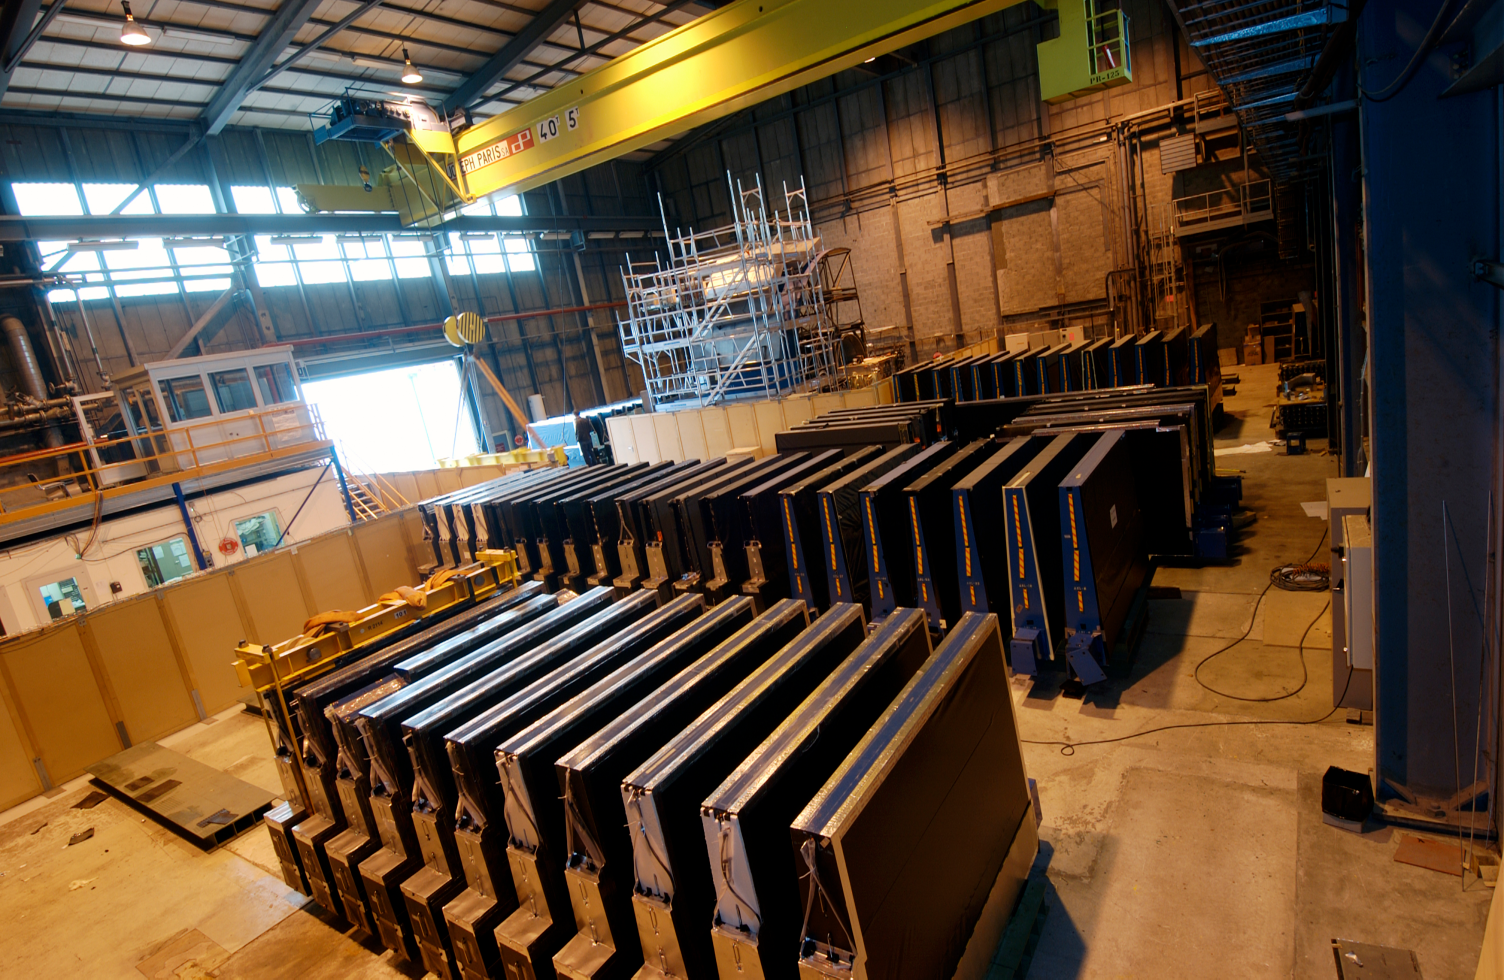
\includegraphics[width=0.495\textwidth]{figures/atlas/tile_pic.pdf}}
\caption{(a) Schematic representation of a TileCal module and its interface with the optical readout. (b)}
\label{fig:atlas:tile}
\end{figure}

An approximately projective geometry, shown in Fig. \ref{fig:atlas:tile_cells}, is provided by the grouping of the readout fibres into the PMTs: this defines a cell structure, and each cell has dimension $\Delta\eta \times \Delta\phi = $ 0.1 $\times$ 0.1 in the first two layers and $\Delta\eta \times \Delta\phi = $ 0.2 $\times$ 0.1 in the third layer. Special cells cover the gap region between the LB and the EB: the gap scintillators in the pseudorapidity region 1.0$<|\eta|<$1.2 and crack scintillators in the region 1.2$<|\eta|<$1.6, in front of the LAr end caps.

\begin{figure}[ht]
\centering
\subfigure{\includegraphics[width=0.7\textwidth]{figures/atlas/tile_cells.pdf}}
\caption{Layout of the projective geometry of the TileCal cells.}
\label{fig:atlas:tile_cells}
\end{figure}

The HEC shares the same cryogenic system as the ECal end caps, and covers the region with 1.5$<|\eta|<$3.2. Liquid argon is more resistant to radiation than the plastic scintillator used in TileCal, and is therefore the preferred choice in the end-cap region. Each side of the HEC consists of two wheels with outer radius of 2.03 m, and each wheel is composed by 32 identical modules. The electromagnetic signal produced in the LAr is collected by catodes on the plates. 

The FCal provides coverage in the forward region with 3.1$<|\eta|<$4.9. The FCal modules are located at high pseudorapidity, at a distance of 4.7 m along the $z$-axis from the interaction point.


\subsection{Muon Spectrometer}

\begin{figure}[ht]
\centering
\subfigure{\includegraphics[width=0.65\textwidth]{figures/atlas/muon}}
\caption{Layout of the ATLAS muon system. Figure from Ref. \cite{atlas:atlas}}
\label{fig:atlas:muon}
\end{figure}

\subsection{Luminosity Detectors}

\subsection{Luminosity Determination and Uncertainty}

\subsection{Trigger System}
\label{sec:cern:trigger}

\subsection{ATLAS Performance Summary}


